\documentclass[11pt,a4paper]{article}

\usepackage[margin=2.5cm]{geometry}
\usepackage{amsmath}
\usepackage{booktabs}
\usepackage{tikz}
\usetikzlibrary{arrows.meta}
\usepackage{graphicx}
\usepackage{float}
\usepackage{tabularx}
\usepackage{array}
\usepackage{enumitem}
\usepackage{totcount}
\usepackage{fancyhdr}
\usepackage{lastpage}
\usepackage{needspace}
\setlength{\emergencystretch}{1.5em}
\usepackage{tocloft}
\usepackage[hidelinks]{hyperref}

% Room for "1.0" style numbers in the contents; list down to 1.1 level only.
\setlength{\cftsecnumwidth}{2.4em}
\setlength{\cftsubsecindent}{2.4em}
\setlength{\cftsubsecnumwidth}{2.4em}
\setcounter{tocdepth}{2}
\tocloftpagestyle{fancy}

% Section numbers as in the NASA ConOps outline: 1.0, 1.1, 1.1.1
% [1, App. S, pp. 251--253].
\renewcommand{\thesection}{\arabic{section}.0}
\renewcommand{\thesubsection}{\arabic{section}.\arabic{subsection}}
\renewcommand{\thesubsubsection}{\thesubsection.\arabic{subsubsection}}

% Controlled-document header on every page.
\newcommand{\docref}{Reference TBD}
\newcommand{\docrev}{Issue 1, Rev.~0 --- DRAFT}
\pagestyle{fancy}
\fancyhf{}
\lhead{\small Remote Controller with Fail-Safe Update --- ConOps}
\rhead{\small \docrev}
\lfoot{\small \docref}
\rfoot{\small Page \thepage\ of \pageref{LastPage}}

% Open items. TBD = not known. TBR = proposal awaiting the author's acceptance
% [1, App. C, pp. 197--198]. Defined once in App. C; totals counted, not typed.
\newtotcounter{tbd}
\newtotcounter{tbr}
\newtotcounter{tbropen}
\newtotcounter{tbdopen}
\newcommand{\tbditem}[2]{\refstepcounter{tbd}\stepcounter{tbdopen}\label{tbd:#1}\item[TBD-\thetbd] #2}
\makeatletter
\newcommand{\tbdresolvedat}[3]{\protected@edef\@currentlabel{#2}\label{tbd:#1}\item[TBD-#2] #3}
\makeatother
\newcommand{\tbritem}[2]{\refstepcounter{tbr}\stepcounter{tbropen}\label{tbr:#1}\item[TBR-\thetbr] #2}
\newcommand{\tbrresolved}[2]{\refstepcounter{tbr}\label{tbr:#1}\item[TBR-\thetbr] #2}
\newcommand{\tbd}[1]{\mbox{\textbf{[\hyperref[tbd:#1]{TBD-\ref*{tbd:#1}}]}}}
\newcommand{\tbr}[1]{\mbox{\textbf{[\hyperref[tbr:#1]{TBR-\ref*{tbr:#1}}]}}}

\setlist[description]{style=multiline,leftmargin=2cm,nosep,font=\normalfont\bfseries}
\setlist[enumerate]{nosep}
\setlist[itemize]{nosep}

\begin{document}

% ---------------------------------------------------------------- cover page
\thispagestyle{fancy}
\begin{center}
{\LARGE\bfseries Remote Controller with Fail-Safe Update\par}
\vspace{0.4em}
{\Large Concept of Operations\par}
\vspace{1em}
\begin{tabular}{@{}ll@{}}
Reference & TBD \tbd{ref} \\
Issue / revision & Issue 1, Revision 0 --- DRAFT \\
Date & 10 October 2026 \\
Author & Andrew Toma \\
Open items & \total{tbdopen} TBD, \total{tbropen} TBR (App.~C) \\
\end{tabular}
\end{center}

\subsection*{Document change record}
\begin{tabular}{@{}lllp{10cm}@{}}
\toprule
Issue & Rev. & Date & Change \\
\midrule
1 & 0 & 2026-10-10 & First draft \\
\bottomrule
\end{tabular}

\tableofcontents

\newpage
% ===========================================================================
\section{Introduction}

\subsection{Project Description}

\subsubsection{Background}
\noindent\textbf{Purpose:} The System lets an operator on the ground command,
monitor, and update a controller in space that nobody can reach, and keeps that controller working between contacts.

\medskip
\noindent\textbf{Need:} A controller that nobody can reach must stay operable,
observable, and correctable for its whole life. Operation, observability, and
maintenance including in-flight modification over the specified lifetime are
three areas a space software specification must cover
[3, Annex~B, items 5.11--5.13, p.~113].

\medskip
\noindent\textbf{Worst-Case Failure:} A failed update can leave the controller
unable to run any firmware and unable to accept new firmware. Without physical
access, that state is permanent.

\medskip
\noindent\textbf{Rationale:} The loss has happened. NASA records a mission
terminated after an in-flight software upload omitted a patch for a defective
countdown timer; its recommendations include test-bed verification of in-flight
software updates [4, Lesson 0559, p.~199].

\subsubsection{Assumptions and Constraints}
\begin{description}
\item[C-1] The ground cannot talk to the controller directly. Every command,
  report, and firmware image passes through the onboard computer.
\item[C-2] All software is built to NASA's software engineering requirements.
  Rigor per part is set by its software class [5, Sec.~3.5.1, p.~24; App.~C].
\item[C-3] One engineer builds and checks the System. No independent team
  reviews the work.
\item[C-4] The System runs on commercial development boards, not on spacecraft
  hardware. It can show how the System behaves, not that it would survive
  launch or space.
\item[A-1] Once launched, physical access to the onboard computer or controller
  is impossible; all fixes and updates must arrive by radio.
\item[A-2] The controller can lose power at any moment, even halfway through
  writing new firmware. The System must survive that without losing the
  controller [2, App.~A, Table~2, p.~63].
\item[A-3] The ground can reach the spacecraft only during line-of-sight
  contact windows \tbd{window}. Between contacts the System must work on its
  own.
\item[A-4] One person operates the ground station. No second person checks a
  command before it is sent, so the System itself must refuse wrong commands.
\item[A-5] Radiation in space can flip single bits in memory, so stored
  firmware can change on its own. The System must not run firmware that has
  changed [2, App.~A, Table~2, p.~63].
\end{description}

\medskip
{\itshape \noindent\textbf{Note.} A constraint (C) is a limit the System must work
within; it is imposed, not chosen. An assumption (A) is a condition taken as
true without proof; the design depends on it, and if it proves false the design
may be wrong. \textbf{[TBR-$n$]} marks a proposal the author has not yet
accepted; \textbf{[TBD-$n$]} marks a value not yet known. Both are listed in
App.~C.\par}

\subsection{Overview of the Envisioned System}

\subsubsection{Overview}
The System comprises two spatially separated operational segments. The
\textbf{ground segment} on Earth includes the operator, the mission operations
center running ground software, and the ground station antenna
[6, Sec.~11.2, p.~305]. The \textbf{space segment} in orbit consists of the onboard
computer and the controller, which operate without physical access.

Communication between segments is strictly established via a radio link during
line-of-sight contact windows \tbd{window}. Outside contact windows, the space
segment operates autonomously. Within the spacecraft, the onboard computer
communicates with the controller over the data link during normal operation.
If the controller's main firmware fails to execute, the onboard computer
utilizes the reprogramming link to restore functional firmware independently of
the controller's primary software. Figure~\ref{fig:segments} illustrates this
segment layout.

\begin{figure}[H]
\centering
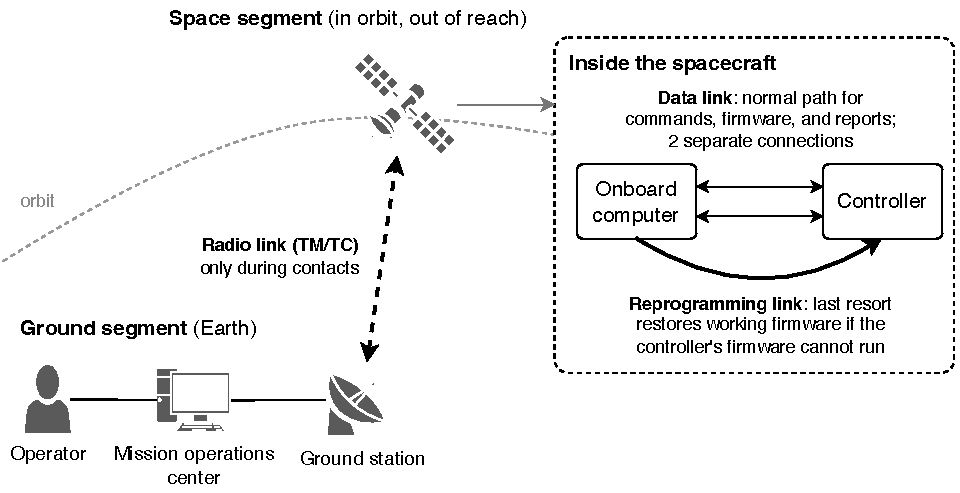
\includegraphics[width=\textwidth]{fig-segments.pdf}
\caption{Ground and space segments, joined only by the radio link during
contact windows. Inside the spacecraft, the data link handles normal
communication, while the reprogramming link restores working firmware if the
controller's firmware cannot run.}
\label{fig:segments}
\end{figure}

\subsubsection{System Scope}
The system context defines the boundary of the System: the system of interest,
its users, and the external elements that interface with it
[7, Sec.~8.3, p.~24].

\begin{table}[H]
\centering
\begin{tabular}{@{}ll@{}}
\toprule
Context Element & System Boundary \\
\midrule
System of Interest & Onboard computer, controller, ground software in the MOC \\
Users & Ground operator \\
External Elements & Radio equipment, spacecraft power supply \\
\bottomrule
\end{tabular}
\end{table}

\begin{itemize}
\item \textbf{Enabling systems:} firmware build tools and bench test setups
  required for development and verification, external to operational scope.
\item \textbf{In scope:} commanding, telemetry, firmware updates, and autonomous
  fault handling between contact windows \tbr{faults}.
\item \textbf{Out of scope:} onboard computer software updates \tbr{obcupdate},
  and the radio equipment, which is used as given.
\end{itemize}

% ===========================================================================
\section{Documents}

\subsection{Applicable Documents}
[1] NASA, \emph{NASA Systems Engineering Handbook}, NASA/SP-2016-6105 Rev~2,
2016. This outline follows its App.~S, pp.~251--253, tailored per its
Sec.~3.11.1, p.~34: Section~7.0 not applicable; App.~C added for open items per its
App.~C, pp.~197--198.

\subsection{Reference Documents}
[2] NASA, \emph{Software Assurance and Software Safety Standard},
NASA-STD-8739.8B, 2022. Off-nominal scenarios cite App.~A, Table~2.

\noindent [3] ESA, \emph{Space engineering --- Software}, ECSS-E-ST-40C Rev.~1,
30 April 2025.

\noindent [4] NASA, \emph{Fault Management Handbook}, NASA-HDBK-1002, Draft~2,
2 April 2012. A draft, not a released standard.

\noindent [5] NASA, \emph{NASA Software Engineering Requirements}, NPR 7150.2D.

\noindent [6] NASA, \emph{State-of-the-Art of Small Spacecraft Technology},
Chapter 11, ``Ground Data Systems and Mission Operations'', 2026 edition.
Ground system architecture in Sec.~11.2 and Fig.~11.2, pp.~305--306.

\noindent [7] NASA, \emph{NASA Systems Modeling Handbook for Systems Engineering},
NASA-HDBK-1009A, 12 March 2025.

% ===========================================================================
\section{Description of Envisioned System}

\subsection{Needs, Goals and Objectives}
\label{sec:ngo}
\begin{description}
\item[NEED] A controller that nobody can reach must stay operable, observable
  and correctable for its whole life.
\item[G-1] \textbf{Operability:} the controller keeps running and acts on the
  operator's commands.
  \begin{itemize}[leftmargin=1.2cm]
  \item[\textbf{O-1}] Every valid operator command is executed. Valid means from the
    operator, allowed in the current state, with possible values, and not
    expired.
  \item[\textbf{O-2}] Firmware and commands not from the operator are never acted on.
  \item[\textbf{O-3}] With one data-link connection lost, commands, telemetry and
    updates continue.
  \item[\textbf{O-4}] No fault found between contacts goes unreported \tbr{faults}.
  \end{itemize}
\item[G-2] \textbf{Observability:} the ground can know what the System is
  doing, how healthy it is, and what happened between contacts.
  \begin{itemize}[leftmargin=1.2cm]
  \item[\textbf{O-5}] No report is lost without the ground being told.
  \end{itemize}
\item[G-3] \textbf{Correctability:} the controller's firmware can be replaced
  for its whole life without losing the controller.
  \begin{itemize}[leftmargin=1.2cm]
  \item[\textbf{O-6}] No update, even one interrupted by a single fault, leaves the
    controller without runnable firmware.
  \end{itemize}
\end{description}

\subsection{Overview of System and Key Elements}
\begin{description}[leftmargin=4.4cm]
\item[Operator] The user. Decides and sends commands, releases new firmware,
  and reads the reports.
\item[Ground software] In the mission operations center. Turns the operator's
  decisions into commands and firmware ready to send, checks them before they
  leave, and keeps every report received.
\item[Onboard computer] Checks commands and firmware and passes them to the
  controller, stores the controller's reports between contacts, watches the
  controller, and restores it when its firmware cannot run.
\item[Controller] Runs its firmware, acts on commands, reports its state, and
  returns to working firmware on its own when new firmware fails.
\end{description}
The ground station's radio equipment and the spacecraft power supply are
outside the System; it uses them as given.

\subsection{Interfaces}
\noindent\textbf{External interfaces}
\begin{description}[leftmargin=4.4cm]
\item[Operator interface] Human. Ground software to operator. Allows the
  flight operator to issue telecommands, authorize firmware deployments, and
  monitor system telemetry.
\item[Radio link] Radio frequency. Ground software to onboard computer via
  external radio equipment. Provides intermittent telemetry and telecommand
  (TM/TC) transfer exclusively during contact windows.
\item[Power] Electrical. Spacecraft power subsystem to onboard computer and
  controller. Subject to unannounced power interruptions at any time
  (assumption A-2).
\end{description}

\medskip
\noindent\textbf{Interfaces between elements}
\begin{description}[leftmargin=4.4cm]
\item[Data link] Digital data. Onboard computer to controller. Nominal
  interface for commands, telemetry, and firmware updates while controller
  firmware is running. Uses two separate connections, so a single connection
  failure does not interrupt operations.
\item[Reprogramming link] Digital data. Onboard computer to controller.
  Recovery interface used as a last resort to restore functional firmware
  independently of the controller's main software.
\end{description}

\subsection{Modes of Operations}
\noindent\textbf{Life-cycle modes of the System}
\begin{description}[leftmargin=3cm]
\item[Test] Ground bench execution with simulated radio link degradation and
  intentional fault injection to demonstrate operational scenarios.
\item[Operation] Active mission execution using the controller modes detailed
  below.
\item[Disposal] Not applicable; limited to bench demonstration scope.
\end{description}

\medskip
\noindent\textbf{Controller modes during operation}
\begin{description}[leftmargin=3cm]
\item[OPERATE] Nominal state executing confirmed firmware. New firmware images
  can be staged in the background during execution \tbr{receive}.
\item[TRIAL] Entered upon transitioning to updated firmware. Executes the new
  image for a bounded evaluation window \tbd{trialtime}. If the new image is
  judged good, the update is committed and the controller returns to OPERATE;
  if not, it enters FALLBACK.
\item[FALLBACK] Entered following a failed firmware trial or boot failure.
  Reverts execution to the previous known-good firmware image or the
  last-resort firmware.
\item[RECOVERY] Entered when no operational firmware image can be executed.
  Controller software execution is halted while the onboard computer restores
  functional firmware via the reprogramming link.
\end{description}

\subsection{Proposed Capabilities}
\noindent\textbf{Telemetry} (serves G-2 Observability)
\begin{description}[leftmargin=3cm]
\item[Capability-1] Generate periodic health reports detailing operational
  status, active firmware version, uptime, reset cause, and thermal telemetry.
\item[Capability-2] Generate asynchronous event-driven reports immediately upon
  significant state changes or operational events.
\item[Capability-3] Apply time tags to all generated telemetry reports.
\item[Capability-4] Store telemetry reports during out-of-contact periods for
  downlink during subsequent contact windows, including notification of any
  unrecoverable telemetry data loss.
\item[Capability-5] Monitor and report health status for each connection of the
  data link.
\end{description}

\medskip
\noindent\textbf{Command handling} (serves G-1 Operability)
\begin{description}[leftmargin=3cm]
\item[Capability-6] Execute telecommands originating exclusively from the authorized ground operator and reject replay attacks.
\item[Capability-7] Acknowledge command reception, disposition (executed or rejected with cause), and completion status for every incoming telecommand.
\item[Capability-8] Reject telecommands invalid for the current operational mode.
\item[Capability-9] Run a repeated telecommand only once.
\item[Capability-10] Enforce a two-step ``arm and execute'' protocol for critical operations.
\item[Capability-11] Reject telecommands containing out-of-bounds parameter values.
\item[Capability-12] Allow the operator to abort an in-progress firmware update while preserving current operational firmware.
\item[Capability-13] Support time-tagged command execution and reject expired commands.
\item[Capability-14] Maintain a command log recording all incoming telecommands and execution responses.
\end{description}

\medskip
\noindent\textbf{Fault handling} (serves G-1 Operability) \tbr{faults}
\begin{description}[leftmargin=3cm]
\item[Capability-15] Detect controller unresponsiveness and initiate autonomous
  recovery sequences.
\item[Capability-16] Automatically fail over to the redundant data-link connection
  upon single-path failure.
\item[Capability-17] Restart crashed onboard processes and continue where they
  stopped.
\item[Capability-18] Log all detected fault events and executed recovery actions for
  subsequent downlink.
\end{description}

\medskip
\noindent\textbf{Update} (serves G-3 Correctability)
\begin{description}[leftmargin=3cm]
\item[Capability-19] Support reliable firmware image reception across intermittent
  radio contact windows.
\item[Capability-20] Validate firmware integrity, source authentication, target
  compatibility, and version policy (preventing unauthorized rollbacks).
\item[Capability-21] Transfer validated firmware images to the controller.
\item[Capability-22] Transition execution to newly uploaded firmware, with the
  activation trigger and scheduling criteria \tbd{switch}.
\item[Capability-23] Evaluate new firmware operational validity post-boot; who
  judges is open \tbd{confirm}.
\item[Capability-24] Automatically roll back to operational firmware if trial
  evaluation fails, without ground intervention.
\item[Capability-25] Downlink firmware update outcome reports to the ground
  segment.
\end{description}

\medskip
\noindent\textbf{Test} (verification only)
\begin{description}[leftmargin=3cm]
\item[Capability-26] Provide controlled, deliberate radio link degradation during
  bench testing.
\item[Capability-27] Support command-driven injection of power interrupts and
  data-link disconnection faults \tbr{faultinject}.
\end{description}

\medskip
\noindent\textbf{Disposal:} none; operational scope limited to bench
demonstration.

% ===========================================================================
\section{Physical Environment}
This section specifies the environment the System encounters across its life
cycle, encompassing simulated mission operations and laboratory integration
and testing. For each environmental condition, the expected system response is
defined as nominal operation, degraded performance tolerance, or survivability
[1, App.~S, p.~252].

\begin{table}[H]
\centering
\begin{tabularx}{\textwidth}{@{}l>{\raggedright\arraybackslash}Xll@{}}
\toprule
Phase & Environmental condition & Response & Shown on bench \\
\midrule
Operation & Thermal range \tbd{temp} & OPERATE & NO \\
Operation & Vacuum & OPERATE & NO \\
Operation & Radiation: single-event upset / memory bit errors & OPERATE & SIMULATED \\
Operation & Electrical: power interruption at any instant & SURVIVE & YES \\
Launch & Mechanical: vibration and launch loads & OPERATE & NO \\
Integration and Test & Laboratory bench: ambient room temperature and pressure & OPERATE & YES \\
\bottomrule
\end{tabularx}
\end{table}

\noindent\textbf{Legend: response}
\begin{description}[leftmargin=3.2cm]
\item[OPERATE] All functions continue normally.
\item[TOLERATE] Partial functional degradation occurs, but no function is
  permanently lost.
\item[SURVIVE] Operational functions temporarily halt and automatically recover
  upon removal of the condition.
\end{description}

\medskip
\noindent\textbf{Legend: shown on bench}
\begin{description}[leftmargin=3.2cm]
\item[YES] The condition itself is reproduced on the bench.
\item[SIMULATED] The condition's effect is injected on purpose; the condition
  itself is not reproduced.
\item[NO] Beyond what bench hardware can show (constraint C-4).
\end{description}

\medskip
\noindent\textbf{Transportation:} not applicable; system transportation is
outside the scope of bench demonstration.

% ===========================================================================
\section{Support Environment}
Firmware is built and released on the ground and sent up during contacts, one
transfer across several if needed. The onboard computer keeps the last
known-good firmware. Update rate \tbd{frequency}. Nothing is repaired after
deployment.

% ===========================================================================
\section{Operational Scenarios}
Every scenario below is demonstrated on hardware and recorded.

\subsection{Nominal Conditions}
\begin{description}[leftmargin=3cm]
\item[Scenario-100] Update: release, upload over one or more contacts, check,
  transfer \tbr{receive}, switch \tbd{switch}, judged good \tbd{confirm},
  confirmed, outcome reported.
\item[Scenario-110] Telemetry: reports stamped and stored between contacts, all sent
  at the next one.
\item[Scenario-120] Scheduled command: received during a contact, runs at its time,
  answer sent at the next contact.
\end{description}

\subsection{Off-Nominal Conditions}
Trigger, then expected outcome. Sources in brackets are items of [2, App.~A,
Table~2].
\begin{description}[leftmargin=3cm]
\item[Scenario-200] Ground link lost mid-transfer: resumes next contact where it
  stopped.
\item[Scenario-210] Command not from operator or replayed: refused, logged [2, p.~62].
\item[Scenario-220] Answer lost, command resent: not run again, ``already done''.
\item[Scenario-230] Command wrong for current state: refused with reason [2, p.~63].
\item[Scenario-240] Impossible value: refused with reason [2, p.~62].
\item[Scenario-250] Dangerous command not armed: refused with reason.
\item[Scenario-260] Command expired: refused with reason [2, p.~63].
\item[Scenario-270] Report storage full: ground told how many were lost.
\item[Scenario-300] Firmware damaged in transfer: refused before the controller
  [2, p.~63].
\item[Scenario-310] Firmware not from operator: refused.
\item[Scenario-320] Firmware below minimum version: refused.
\item[Scenario-330] Firmware for another controller: refused [2, p.~63].
\item[Scenario-340] Power lost during firmware write: previous firmware runs; retry
  possible [2, p.~63].
\item[Scenario-350] New firmware hangs: back to previous, unaided.
\item[Scenario-360] New firmware restart loop: back to previous after \tbd{bootcount}
  starts [2, p.~64].
\item[Scenario-370] New firmware never judged good: back to previous.
\item[Scenario-380] Previous firmware also bad: last-resort firmware runs.
\item[Scenario-390] Operator cancels update: known-good firmware left running.
\item[Scenario-400] Bit error in stored firmware: detected, not run \tbr{bitflip}
  [2, p.~63].
\item[Scenario-410] No firmware can run: restored through the reprogramming link
  [2, p.~63].
\item[Scenario-500] One data-link connection fails: everything continues on the
  other; reported.
\item[Scenario-510] Both data-link connections fail: controller keeps working; loss
  reported; reprogramming link still usable \tbr{bothlinks}.
\item[Scenario-520] Controller silent: noticed, recovery tried, recorded
  \tbr{faults}.
\item[Scenario-530] Onboard program crash: it restarts and resumes any update; the
  controller is unaffected \tbr{faults}.
\end{description}

% ===========================================================================
\section{Impact Considerations}
Not applicable: bench demonstration.

% ===========================================================================
\section{Risks and Potential Issues}
\begin{description}
\item[R-1] Both data-link connections may share software; one defect could cut
  both.
\item[R-2] Controller memory may not hold last-resort plus two working firmwares.
\item[R-3] Second data-link connection and reprogramming link not yet shown on
  bench.
\item[R-4] Demonstration date \tbd{date}; undemonstrated scenarios are declared,
  not dropped.
\end{description}

% ===========================================================================
\appendix
\renewcommand{\thesection}{\Alph{section}}

\section{Acronyms}
\begin{description}[leftmargin=2.2cm]
\item[ConOps] Concept of Operations
\item[MOC] Mission operations center
\item[TBD] To Be Determined
\item[TBR] To Be Resolved
\item[TC] Telecommand
\item[TM] Telemetry
\end{description}

\section{Glossary}
\begin{description}[leftmargin=3.2cm]
\item[Confirmed] Firmware judged good after its trial; only confirmed firmware
  is known-good.
\item[Last-resort] Known-good firmware that updates never replace (golden
  image).
\item[Switch] The controller stops running old firmware and starts the new.
\item[Arm] First step of a dangerous command; changes nothing alone.
\item[Expiry] Time after which a waiting command is refused.
\end{description}

\section{Open Items}
Unmarked statements were stated or accepted by the author on 9--10 October
2026. TBR items are resolved before the hazard analysis.
\subsection*{Resolved}
\begin{description}
\tbrresolved{situation}{Spacecraft controller, ground contacts only, no
  physical access, bench stand-in, bit errors occur, no repair. Accepted by the
  author, 10 October 2026.}
\tbrresolved{power}{Controller power can drop at any instant, including
  mid-write. Accepted by the author, 10 October 2026.}
\tbrresolved{operator}{One operator. Accepted by the author, 10 October 2026.}
\tbrresolved{telemetry}{Capability-1, Capability-2, Capability-3 and Capability-5 as
  written. Accepted by the author, 10 October 2026.}
\end{description}

\subsection*{Open}
\begin{description}
\tbritem{faults}{O-4 and Capability-15 to Capability-18 as written (shown 10 Oct, not yet
  accepted).}
\tbritem{receive}{Controller keeps working while new firmware arrives.}
\tbritem{obcupdate}{Onboard computer's own update out of scope.}
\tbritem{bothlinks}{Reprogramming link still usable with both data-link
  connections lost.}
\tbritem{bitflip}{Stored firmware checked before start; damaged copy skipped.}
\tbritem{faultinject}{Test setup can cut power and break one connection.}
\tbditem{ref}{Project name and document reference.}
\tbditem{date}{Demonstration date.}
\tbditem{switch}{Switch automatically on arrival, or only on operator command.}
\tbditem{confirm}{Who judges new firmware good: controller or operator.}
\tbditem{window}{Contact window length and gap (sourced, or a test parameter).}
\tbditem{trialtime}{Trial time limit (requirements).}
\tbditem{bootcount}{Failed starts before going back (requirements).}
\tbditem{frequency}{Update rate.}
\tbditem{temp}{Temperature range.}
\end{description}

\end{document}
